\section{The ratchet, I: the decomposition oracle}\label{sec:oracle}

Figure~\ref{fig:ratchet} plots every improvement in the ledger as
candidate/incumbent on a log scale. Table~\ref{tab:ledger} (in
\S\ref{sec:families}) gives each one's class, boundary and source. This
section covers the oracle, $C_{\mathrm{dec}}$ in~\eqref{eq:cost}.

\begin{figure}[p]
\centering
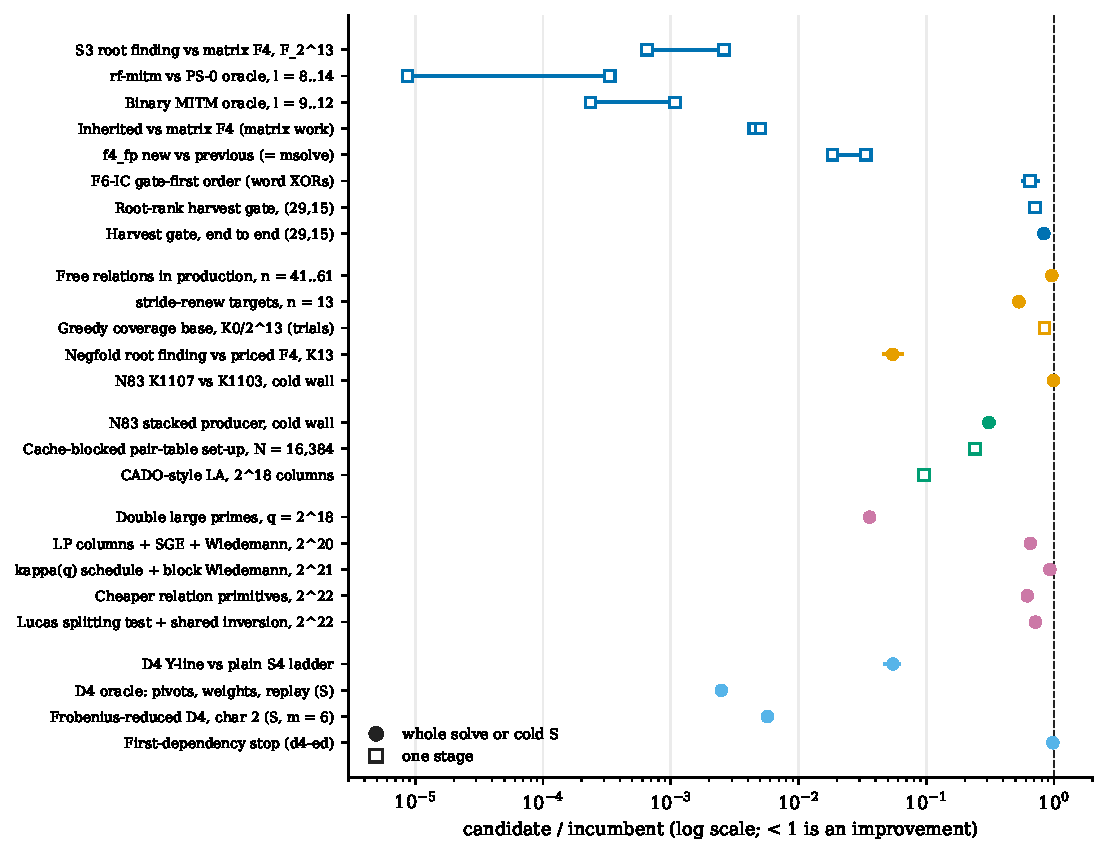
\includegraphics[width=\linewidth]{figures/fig-ratchet.pdf}
\caption[]{The ratchet. Each row is one change, candidate/incumbent on the
study's own boundary; less than 1 is an improvement. Filled circles are
whole solves or cold $S$; open squares are single stages. Bars show 95\%
intervals. Rows with two markers show the range a source reports across
instances, not an interval. Rows are grouped by pipeline term and are not
comparable across groups: incumbents, curves and units differ. Values and
sources: \art{papers/ecdlp-ic-improvement-ledger/figures/data.json}.}
\label{fig:ratchet}
\end{figure}

\subsection{Root finding replaces the Gr\"obner solve}

For two summands, the decomposition question has a closed-form answer.
For $E:y^2=x^3+ax+b$ and affine $R,F$ with $x_R\ne x_F$,
\[
  S_3(x_R,x_F,X)=(x_R-x_F)^2\,\bigl(X-x(R+F)\bigr)\bigl(X-x(R-F)\bigr).
\]
So $R=\pm F_i\pm F_j$ if and only if $x(R\mp F_i)\in x(\Fb)$. The identity is
machine-checked in Lean~4 with Mathlib
(\art{papers/rootfinding-decomposition/lean/S3Roots.lean}). The resulting
oracle is one subtraction and one hash probe per base point, with every
inversion batched. For $m=3,4$, a table of pair sums turns a decomposition
into $N$ or $N^2$ probes. The mechanism is the second algorithm of McGuire
and Mueller~\cite{mcguire2017}; what is new here is engineering and
measurement.

Per decomposition, root finding is $383\times$ ($\FF_{2^9}$, $N=55$) and
$1{,}535\times$ ($\FF_{2^{13}}$, $N=4{,}005$) cheaper than matrix F4. Every
verdict agreed with F4. The \texttt{rf-mitm} oracle refutes a binary target
$3{,}007$--$115{,}160\times$ faster than the earlier PS-0 oracle across
$\ell=8..14$ (\art{research/pdp_root_finder_20261012/}). The
meet-in-the-middle oracle on a non-Koblitz curve over $\FF_{2^{37}}$
reached $\ell=12$. It is $928$--$4{,}244\times$ faster than pairs-and-solve
on $\ell=9..12$, with no disagreement on 256 targets
(\art{research/binary_mitm_oracle_l11_l12_20261016/}).

The end-to-end effect is two orders of magnitude smaller than the stage
effect:
\begin{itemize}
\item against msolve, on 16--24-bit prime curves, $50$--$105\times$;
\item on the one binary instance large enough to amortise the table
  ($n=23$), $122\times$; F4 is faster at $n\le13$;
\item inside ecbench at Koblitz $n=13$, a root-finding arm folded over
  negation costs $0.0545$ $[0.047,0.064]$ of an inherited-F4 arm whose
  word XORs are priced (\art{research/ecbench_rootfind_faster_20261014/}).
\end{itemize}
A late correction affects the last comparison. On 20 October a cross-ISA
replay showed that F4's counted word XORs depend on whether the host has
BMI2 (\S\ref{sec:audit}). Once F4 is priced, the root-finding pair table
is about $17$--$22\times$ cheaper than F4 at $n=13$
(\art{research/validation_sweep_20261019/D-known-issues/REPORT.md}). The
direction is unchanged.

\subsection{The Gr\"obner family, where it is still needed}

For $m\ge3$ over binary fields the oracle is still a Gr\"obner solve. Four
changes moved it.
\begin{itemize}
\item \emph{Inherited F4.} Each child node of the DPLL-style tree inherits
  its parent's echelon form. This does $198.6$--$222.1\times$ less matrix
  work than matrix F4 on identical trees. At $m=19$ matrix F4 timed out at
  $1{,}800$\,s, while inherited F4 finished in about 6\,s
  (\art{research/f4_f5_f6_cross_family_20261011/}).
\item \emph{$\FF_p$ F4 at msolve parity.} Gebauer--M\"oller criteria,
  packed monomials and interned symbolic preprocessing made
  \texttt{f4\_fp} $29.8$--$54.1\times$ faster than its predecessor. msolve
  over ours is $0.96$--$1.22$ single-threaded, and every reduced basis
  agrees with Singular or msolve
  (\art{research/f4_fp_msolve_parity_20261011/}). Blocked pair reduction
  then gave $0.78$--$0.89\times$ wall on the quadratic $n=10,11$ systems
  (\art{research/f4_fp_blocked_pairs_20261016/}; L0, descriptive).
\item \emph{Gate-first order in F6-IC.} Checking the factor-base domain
  gate before reduction cuts word XORs by $1.336$--$1.733\times$ and CPU by
  $1.56$--$2.12\times$. All 80 of 80 targets were decided identically
  (\art{research/f6_gate_first_x86_20261016/}). It is now the default. An
  arm64 rerun on 22 October found that turning it off costs
  $1.62$--$2.15\times$, so every default stands
  (\art{research/arm64_f4_defaults_20261022/README.md}; shared CI VMs, one
  run each).
\item \emph{Harvesting what the oracle discarded.} Linear rows that the
  Gr\"obner oracle used to throw away are kept: $0.858$ $[0.803,0.916]$ at
  $(n,\ell)=(23,12)$, where the gate fires. A root-rank gate then made the
  harvest fire on more cells: $1.41\times$ $[1.32,1.52]$ CPU at $(29,15)$,
  $1.89\times$ at $(37,19)$, and $1.20\times$ and $1.14\times$ end to end
  at $(29,15)$ and $(31,16)$, with 0 of 248 root-set failures
  (\art{research/ic_improve3_20261015/02-harvest-gate}).
\end{itemize}

\paragraph{Changes that did not count.}
\begin{itemize}
\item \emph{F6-IC as a frontier move.} F6-IC uses $0.77$--$0.82$ of
  inherited F4's word XORs. Once its batched group additions are charged,
  though, its $S$ is $64.6$--$1{,}353\times$ inherited F4's. That is
  \cls{accounting}.
\item \emph{Algebraic oracles against the MITM floor.} No algebraic oracle
  (inherited F4, F6-IC, SAT, split-$S_4$ hybrids, a chained-$S_3$ solver)
  grows more slowly in $n$ than the meet-in-the-middle floor. The cheapest
  is $3.0\cdot10^2\times$ the floor at $n=13$ and $3.8\cdot10^4\times$ at
  $n=31$ for $m=3$ (\art{research/ic_m3_algebraic_vs_mitm_20261014/}).
\item \emph{Root-shape replay in inherited F4.} It regresses by
  $1.015$--$1.328\times$, so the switch stays off
  (\art{research/pdp_shape_replay_20261015/}).
\item \emph{F4 trace replay in the Jacobian-cover pipeline.} It now costs
  $+31\%$ and $+35\%$ (\art{research/ic_cover_leads_20261018/README.md}).
\end{itemize}

\paragraph{Reading.} The oracle is the term the programme improved most:
by two to five orders of magnitude where root finding applies, and by one to
two orders in counted matrix work where Gr\"obner bases are still needed.
None of this changes the trial count $m!\,r/N^{m-1}$. That is why the
remaining sections deal with $N$, the yield, set-up and linear algebra.
